\documentclass[11pt]{article}

% Preamble!!
\usepackage{titling}
\setlength{\voffset}{0.7in}
\setlength{\droptitle}{-10em}
\usepackage{titlesec}
\titlelabel{\thetitle.\quad}
\usepackage{xcolor}
\usepackage{adjustbox}
\usepackage{amsmath, amsthm, amsfonts, amssymb}
\usepackage{graphicx}
\usepackage{setspace}
\usepackage{longtable}
\usepackage{breqn}
\usepackage{lscape}
\usepackage{indentfirst}
\usepackage[labelsep=period,justification=justified,singlelinecheck=false,font = footnotesize, labelfont=bf]{caption}
\usepackage{booktabs}
\usepackage{tabularx,ragged2e}
\usepackage{natbib}
\usepackage{rotating}
\usepackage{placeins}
\usepackage{subcaption}
\usepackage{hyperref}
\definecolor{burntorange}{rgb}{0.8, 0.33, 0.0}
\hypersetup{
    colorlinks=true,
    linkcolor=orange,
    filecolor=magenta,      
    urlcolor=burntorange,
}
\pagenumbering{arabic}

\usepackage{bbm}
\usepackage[margin=1in]{geometry}

\usepackage{enumerate}
\usepackage{array}
\usepackage[T1]{fontenc}
\usepackage[font=small,labelfont=bf,tableposition=top]{caption}
\usepackage{mathtools}
\newcommand\eho{\stackrel{\mathclap{\small\mbox{$H_0$}}}{=}}
\newcommand\sho{\stackrel{\mathclap{\small\mbox{$*$}}}{=}}
\newcommand\dho{\stackrel{\mathclap{\small\mbox{$d$}}}{=}}
\newcommand\qho{\stackrel{\mathclap{\small\mbox{$?$}}}{=}}

% \usepackage{authblk}


\DeclareCaptionLabelFormat{andtable}{#1~#2  \&  \tablename~\thetable}

\usepackage{fullpage, amsmath, amssymb, amsthm, bbm, color}
\usepackage{graphicx,caption,subcaption,placeins}
\usepackage{dsfont}

\usepackage{natbib}
\bibpunct{(}{)}{;}{a}{,}{,}

\newtheorem{assumption}{Assumption}
\newtheorem{definition}{Definition}
\newtheorem{theorem}{Theorem}
\newtheorem{example}{Example}
\newtheorem{procedure}{Procedure}


\usepackage{tikz}
\usetikzlibrary{positioning,chains,fit,shapes,calc}

\definecolor{myblue}{RGB}{80,80,160}
\definecolor{mygreen}{RGB}{80,160,80}


\begin{document}

\title{FIN 373 Homework 5 \\ {\large due: \textbf{9/28/21}}}
\date{}
\maketitle

\vspace{-20mm}

\noindent Instructions: Please submit solutions on canvas.  Only a knitted pdf of an {\tt Rmarkdown} file will be accepted.
\\

\noindent \textbf{Problem 1:} The paper \href{http://www.stat.columbia.edu/~gelman/research/published/rb_qjps.pdf}{Rich State, Poor State, Red State, Blue State: What's the Matter with Connecticut?} discusses the peculiar trend of Republican voting share's relationship to income within and among states.  See, for example, Figures 3 and 4 in the paper.  Without worrying about the modeling details, describe qualitatively what Figure 4 is showing (the different axes, open and solid circles, etc.).  Why are the lines different slopes on the left panel?  What other variables are potentially driving the difference in these slopes?  Please be as descriptive and specific as possible, either through additional quantitative evidence outside of the paper or developing a testable hypothesis. 

\vspace{7mm}
\noindent \textbf{Problem 2:} The poster below says, ``We don't believe Churov! We believe Gauss!''  Churov is the head of the State Electoral Commissions and Gauss refers to a 18th century German mathematician, Carl Friedrich Gauss, whom the Gaussian (Normal) distribution was named after. 

In this exercise, we use the rules of probability to detect election fraud by examining voting patterns in the 2011 Russian State Duma election. (The State Duma is the federal legislature of Russia.)\footnote{This exercise is based on: \href{https://www.cambridge.org/core/journals/political-analysis/article/detecting-election-fraud-from-irregularities-in-voteshare-distributions/1C48196DDCECC891F913CE0CEE948F3E}{Detecting Election Fraud from Irregularities in Vote-Share Distributions}. \textit{Political Analysis}. Arturas Rozenas (2017). } The ruling political party, United Russia, won this election, but faced many accusations of election fraud, which the Russian government denied.  Some protesters highlighted irregular patterns of voting as evidence of election fraud, as shown in the poster. In particular, protesters pointed out the relatively high frequency of common fractions such as $1/4$, $1/3$, and $1/2$ in the official vote shares.

\begin{center}
	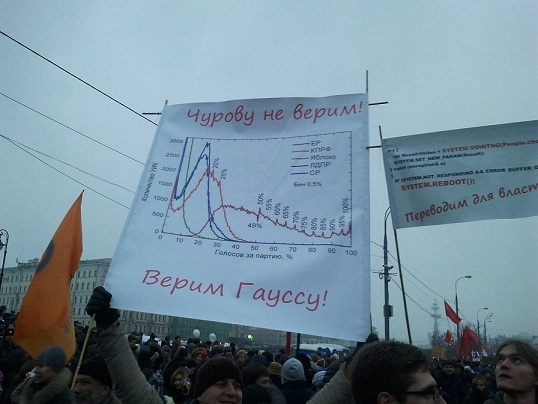
\includegraphics[scale=0.4]{figures/russia-fraud.jpg}	
\end{center}


We use official election results, contained in the {\tt russia2011} data frame in {\tt fraud.RData} to investigate whether there is any evidence for election fraud.  This file can be loaded using the {\tt load} function. In addition to {\tt russia2011}, the file contains election results from the 2003 Russian Duma election {\tt russia2003}, the 2012 Russian presidential election {\tt russia2012}, and the 2011 Canadian election {\tt canada2011} as separate data frames.  Each of these data sets has the same variables, described in the table below.

\vspace{1mm}
\begin{center}
\begin{tabular}{l p{11cm}}
 \hline
\textit{Variable} & \textit{Description} \\
\hline
 {\tt N} &                 Total number of voters in a precinct \\
{\tt turnout} &          Total number of turnout in a precinct \\
{\tt votes} &             Total number of votes for winner in a precinct \\
\hline
\end{tabular}
\end{center}
\begin{enumerate}[a.]
\item To analyze the 2011 Russian election results, first compute United Russia's vote share as a proportion of the voters who turned out.  Identify the 10 most frequently occurring fractions for the vote share.  Create a histogram that sets the number of bins to the number of unique fractions, with one bar created for each uniquely observed fraction, to differentiate between similar fractions like $1/2$ and $51/100$. This can be done by using the {\tt breaks} argument in the {\tt hist} function.  What does this histogram look like at fractions with low numerators and denominators such as $1/2$ and $2/3$?
\item The mere existence of high frequencies at low fractions may not imply election fraud.  Indeed, more numbers are divisible by smaller integers like 2, 3, and 4 than by larger integers like 22, 23, and 24.  To investigate the possibility that the low fractions arose by chance, assume the following probability model:
\begin{itemize}
	\item Turnout for a precinct is binomially distributed, with size equal to the number of voters in the precinct and success probability equal to its observed turnout rate.
	\item Conduct a Monte Carlo simulation under these assumptions. 1000 simulated elections should be sufficient.  (Note that this may be computationally intensive code.  Write your code for a small number of simulations to test before running all 1000 simulations.)
\end{itemize}
What are the 10 most frequent vote share values?  Create a histogram similar to the one in the previous question.  Briefly comment on the results.
\item To judge the Monte Carlo simulation results against the actual results of the 2011 Russian election, we compare the observed fraction of observations within a bin of certain size with its simulated counterpart.  To do this, create histograms showing the distribution of part (b)'s four most frequently occurring fractions, i.e., $1/2$, $1/3$, $3/5$, and $2/3$, and compare them with the corresponding fractions' proportion in the actual election. Briefly interpret the results.
\item We now compare the relative frequency of observed fractions with the simulated ones beyond the four fractions examined in the previous question.  To do this, we choose a bin size of 0.01 and compute the proportion of observations that fall into each bin.  We then examine whether or not the observed proportion falls within the 2.5 and 97.5 percentiles of the corresponding simulated proportions. Plot the result with vote share bin on the horizontal axis and estimated vote share on the vertical axis. This plot attempts to reproduce the one held by protesters in the figure.  Now count the number of times an observed precinct vote share falls outside its simulated interval.  Interpret the results.
\item To put the results of the previous question in perspective, apply the procedure developed in the previous question to the 2011 Canadian elections and the 2003 Russian election, where no major voting irregularities were reported.  In addition, apply this procedure to the 2012 Russian presidential election, where election fraud allegations were reported.  No plot needs to be produced. Briefly comment on the results you obtain.

Note: This question requires computationally intensive code. Write a code with a small number of simulations first and then run the final code with 1000 simulations.
\end{enumerate}


\vspace{7mm}
\noindent \textbf{Problem 3:} Using built-in {\tt R} functions, simulate three random variables that display a confounded relationship.  You are free to choose the distributions these random variables follow, and be sure to provide visual and numerical evidence of confounding.  

\end{document}

